\documentclass[17pt, aspectratio=169]{beamer}

\beamertemplatenavigationsymbolsempty
\usetheme{CambridgeUS}
\usecolortheme{dolphin}
\useinnertheme{rectangles}

\title{M.O.S.I.S Final Report Presentation}
\author[Fabio J. \& Eduardo S.]{Fabio J. Matos Nieves \& Eduardo S. Miranda Figueroa}
\institute[UPRM]{University of Puerto Rico Mayagüez Campus}
\date{December 11, 2023}

\begin{document}
\begin{frame}
	\maketitle
\end{frame}
\begin{frame}
	\tableofcontents
\end{frame}
\section{Introduction}
\subsection*{Background}
\begin{frame}{What is M.O.S.I.S?}
	\begin{columns}
		\column{0.5\textwidth}
		\centering
		\textbf{M.O.S.I.S}\\
		Marine Operated Stereoscopic Imaging System

		\column{0.5\textwidth}
		\centering
		\begin{figure}
			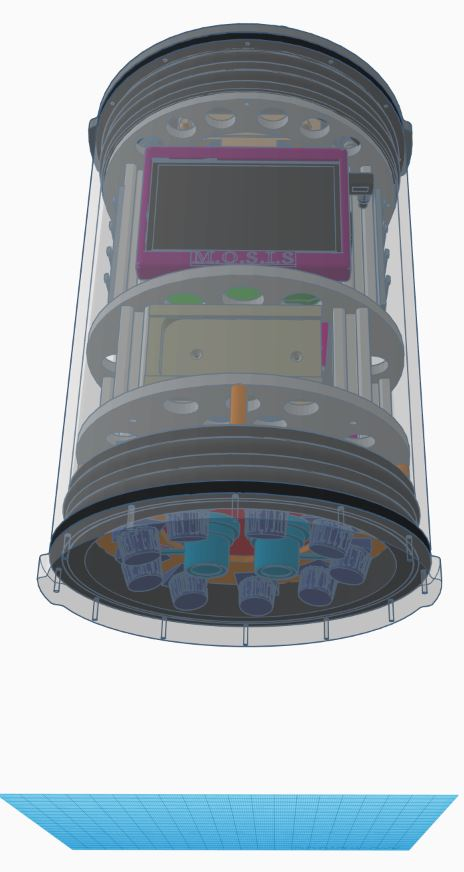
\includegraphics[height=0.85\textheight]{./Figures/M.O.S.I.S_Model.jpeg}
		\end{figure}
	\end{columns}
\end{frame}
\section{Body}
\subsection*{System Specifications}
\begin{itemize}
	\item 400\times400 preview for left and right cameras
	\item Displays temperature, pressure, dissolved oxygen and pH of the environment
	\item User interface navigation using on board buttons
	\item Controls camera parameters and on board lighting
	\item Calibrates pH and dissolved oxygen sensors
\end{itemize}
\subsection*{Testing and Validation}
\subsection*{Design Alternatives}
\subsection*{Diagrams}
\subsection{Video Demo}
\subsection*{Deliverables and Milestones}
\subsection{Project Assessment}
\subsection*{Project Impact}
\subsection*{Expenditure Summary}
\section{Conclusion}
\subsection{Deliverables}
\subsection{Achievements and Lessons Learned}
\end{document}